\chapter{Advanced Algorithms}
\label{chap:advanced_algorithms}

\begin{figure}[ht]
	\hfill
	\begin{minipage}{0.5\textwidth}
		\centering
		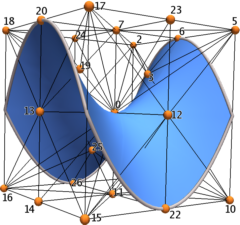
\includegraphics{VTKTextbook-168}
		\caption*{\texttt{An isocontour of a tri--quadratic Lagrange--interpolantion. Image courtesy D. Thompson and P. Pébay Sandia National Labs.}}
	\end{minipage}
\end{figure}

\firstletter{W}e return again to visualization algorithms.
This chapter describes algorithms that are either more complex to implement, or less widely used for 3D visualization applications.
We retain the classification of algorithms as either scalar, vector, tensor, or modelling algorithms.

\section{Scalar Algorithms}

As we have seen, scalar algorithms often involve mapping scalar values through a lookup table, or creating contour lines or surfaces.
In this section, we examine another contouring algorithm, dividing cubes , which generates contour surfaces using dense point clouds.
We also describe carpet plots.
Carpet plots are not true 3D visualization techniques, but are widely used to visualize many types of scalar data.
Finally, clipping is another important algorithm related to contouring, where cells are cut into pieces as a function of scalar value.

\subsection{Dividing Cubes}

Dividing cubes is a contouring algorithm similar to marching cubes \cite{Cline88}. Unlike marching cubes, dividing cubes generates point primitives as compared to triangles (3D) or lines (2D). If the number of points on the contour surface is large, the rendered appearance of the contour surface appears "solid."q To achieve this solid appearance, the density of the points must be at or greater than screen resolution. (Also, the points must be rendered using the standard lighting and shading equations used in surface rendering.)

The motivation for dividing cubes is that rendering points is much faster than rendering polygons. This varies depending upon rendering hardware/software. Special purpose hardware has been developed to render shaded points at high speed. In other systems, greater attention has been placed on polygon rendering, and the rendering speed differences are not so great. Also, certain geometric operations such as clipping and merging data are simple operations with points. Comparable operations with polygons are much more difficult to implement.

One disadvantage of creating contours with dense point clouds is that magnification of the surface (via camera zooming, for example) reveals the disconnected nature of the surface. Thus, the point set must be constructed for maximum zoom, or constructed dynamically based on the relative relationship between the camera and contour.

Although dividing cubes was originally developed for volume datasets, it is possible to adapt the algorithm to other dataset types by subdividing in parametric coordinates. Our presentation assumes that we are working with volumes.

\begin{figure}[!htb]
    \centering
    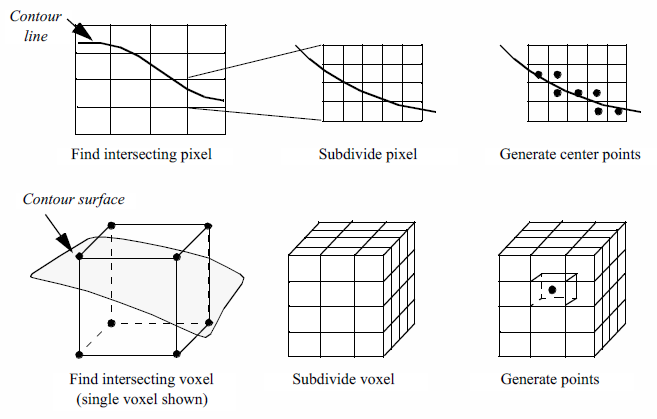
\includegraphics[width=0.98\textwidth]{Figure9-1}\\
    \caption{Overview of the dividing cubes algorithm. Voxels through which the contour passes are subdivided into subvoxels at less than screen resolution. If the contour passes through a subvoxel, a center point is generated.}\label{fig:Figure9-1}
\end{figure}

Figure \ref{fig:Figure9-1} provides an overview of the dividing cubes algorithm. Like other contouring algorithms, we first choose a contour value. We begin by visiting each voxel and select those through which the isosurface passes. (The isosurface passes through a voxel when there are scalar values both above and below the contour value.) We also compute the gradient at each voxel point for use in computing point normals.

After selecting a voxel that the isosurface passes through, the voxel is subdivided into a regular grid of $n1 \times n2 \times n3$ subvoxels. The number of divisions is controlled by the width of a voxel $w_i$ in combination with screen resolution $R$. The screen resolution is defined as the distance between adjacent pixels in world coordinates. We can express the number of divisions ni along the coordinate axes $x_i$ as $w_i$

\begin{equation}\label{eq:9.1}
n_i = \dfrac{w_i}{R}
\end{equation}
\myequations{Number of divisions along a coordinate axis.}

where the quotient is rounded up to the nearest integer. The scalar values at the subpoints are generated using the interpolation functions for a voxel (see Figure \ref{fig:Figure8-10}). Then we determine whether the contour passes through each subvoxel. If it does, we simply generate a point at the center of the subvoxel and compute its normal using the standard interpolation functions.

\begin{figure}[!htb]
    \centering
    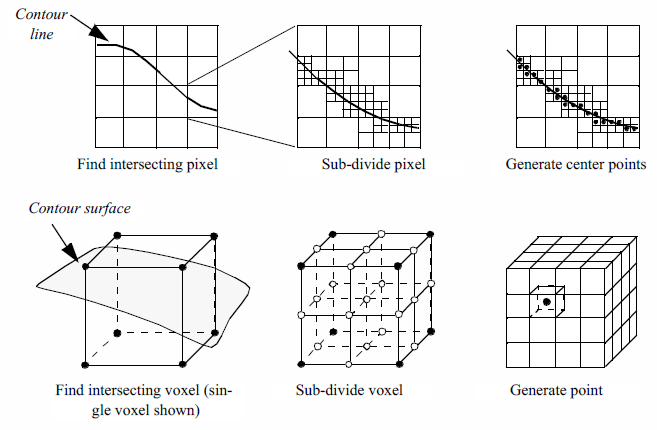
\includegraphics[width=0.98\textwidth]{Figure9-2}\\
    \caption{Recursive dividing cubes algorithm. Top half of figure shows algorithm depicted in two dimensions. Lower half depicts algorithm in three dimensions.}\label{fig:Figure9-2}
\end{figure}

An interesting variation on this algorithm is a recursive implementation as shown in Figure \ref{fig:Figure9-2}. Instead of subdividing the voxel directly (i.e., procedurally) into a regular grid we recursively divide the voxel (similar to octree decomposition). The voxel is subdivided regularly creating eight subvoxels and 19 new points (12 midedge points, 6 midface points, and 1 midvoxel point). The scalar values at the new points are interpolated from the original voxel using the trilinear interpolation functions. The process repeats for each subvoxel if the isosurface passes through it. This process continues until the size of the subvoxel is less than or equal to screen resolution. In this case, a point is generated at the center of the subvoxel. The collection of all such points composes the dividing cube's isosurface.

The advantage of the recursive implementation is that the subdivision process terminates prematurely in those regions of the voxel where the contour cannot pass. On the other hand, the recursive subdivision requires that the voxel subdivision occurs in powers of two. This can generate far more points than the procedural implementation.

\begin{figure}[!htb]
    \centering
    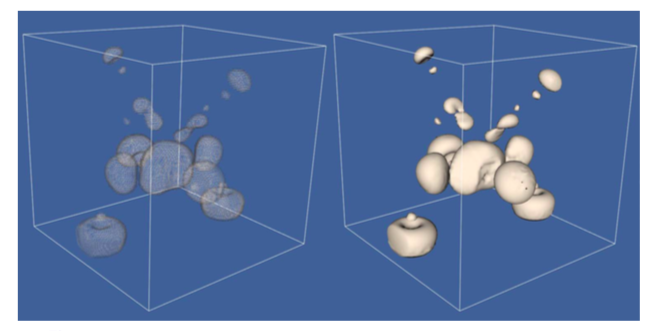
\includegraphics[width=0.98\textwidth]{Figure9-3}\\
    \caption{Examples of dividing cubes isosurface. The left image consists of 50,078 points, and the right image consists of 2,506,989 points.}\label{fig:Figure9-3}
\end{figure}

Figure \ref{fig:Figure9-3} shows two examples of dividing cubes isosurfaces. The contour surface on the left consists of 50,078 points. Because the points are not generated at display resolution, it is possible to see through the contour surface. The second contour surface on the right is composed of 2,506,989 points. The points are generated at display resolution, and as a result the contour surface appears solid.

As Figure \ref{fig:Figure9-1} and Figure \ref{fig:Figure9-2} show, the points generated by dividing cubes do not lie exactly on the contour surface. We can determine the maximum error by examining the size of the terminal subvoxels. Assume that a terminal subvoxel is a cube, and that the length of the side of the cube is given by $l$. Then the maximum error is half the length of the cube diagonal, or $l \sqrt{3} / 2$.

\subsection{Carpet Plots}

A common data form is a 2D image dataset with associated scalar data. Carpet plots can visualize data in this form. A carpet plot is created by warping a 2D surface in the direction of the surface normal (or possibly some user-defined direction). The amount of warping is controlled by the scalar value, possibly in combination with a scale factor. Carpet plots are similar to the vector displacement plots (see ``Displacement Plots'' on page \pageref{subsec:displacement_plots})

Although carpet plots are typically applied to image data, they can be used to visualize datasets composed of 2D structured grids or 2D unstructured grids. In their basic form carpet plots can be used to visualize only three variables: two surface position coordinates and a scalar value. However, it is common to introduce another variable by using color mapping on the surface.

\begin{figure}[!htb]
    \centering
    \begin{subfigure}{0.48\linewidth}
        \centering
        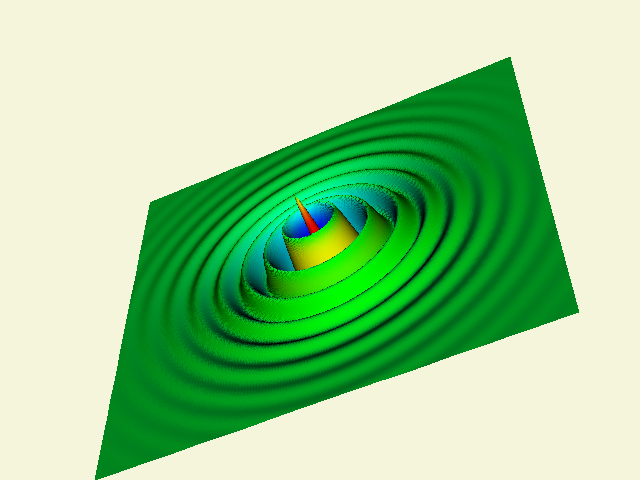
\includegraphics[width=.96\linewidth]{Figure9-4a}
        \caption{Exponential cosine function.(\href{https://lorensen.github.io/VTKExamples/site/Cxx/VisualizationAlgorithms/ExponentialCosine/}{ExponentialCosine.cxx} or \href{https://lorensen.github.io/VTKExamples/site/Python/VisualizationAlgorithms/ExponentialCosine/}{ExponentialCosine.py})}\label{fig:Figure9-4a}
    \end{subfigure}
    \hfill
    \begin{subfigure}{0.48\linewidth}
        \centering
        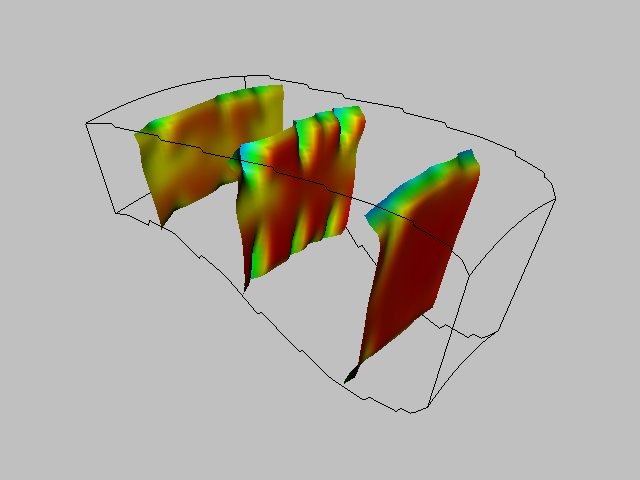
\includegraphics[width=.96\linewidth]{Figure9-4b}
        \caption{Flow energy.(\href{https://lorensen.github.io/VTKExamples/site/Cxx/VisualizationAlgorithms/WarpCombustor/}{WarpCombustor.cxx} or \href{https://lorensen.github.io/VTKExamples/site/Python/VisualizationAlgorithms/WarpCombustor/}{WarpCombustor.py})}\label{fig:Figure9-4b}
    \end{subfigure}%
    \caption{Carpet plot. (a) Visualization of an exponential cosine function. Function values are indicated by surface displacement. Colors indicate derivative values. Carpet plot of combustor flow energy in a structured grid. Colors and plane displacement represent energy values.}
    \label{fig:Figure9-4}
\end{figure}

Figure \ref{fig:Figure9-4} illustrates application of carpet plots. Figure \ref{fig:Figure9-4}(a) shows the exponential cosine function centered at the origin with points located at radius $r$

\begin{equation}\label{eq:9.2}
F(r) = e^{-r}\cos(10\, r)
\end{equation}
\myequations{Exponential cosine function.}

The function values are used to warp the surface while the function derivatives are used to color it. Figure \ref{fig:Figure9-4}(b) shows a carpet plot that visualizes flow energy in a structured grid. Both displacement and color are used to show the energy values. Although this figure is similar to Figure \ref{fig:Figure6-14}(b) there are some important differences. Figure \ref{fig:Figure6-14}(b) displays vector data whereas Figure \ref{fig:Figure9-4}(b) displays scalar data. Figure \ref{fig:Figure9-4}(b) deforms the surface in the direction of surface normal (or possibly a user-defined direction). The vector data (i.e., vector orientation) controls the direction of deformation in Figure \ref{fig:Figure6-14}(b).

\subsection{Clipping With Scalar Fields}

\begin{figure}[!htb]
    \centering
    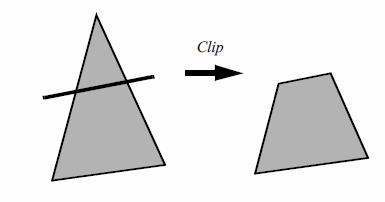
\includegraphics[width=0.98\textwidth]{Figure9-5}\\
    \caption{Clipping a triangle produces a polygon. The dark line represents an infinite plane.}\label{fig:Figure9-5}
\end{figure}


Clipping is a common graphics operation that limits the extent of a polygon so that it does not lie outside the view frustrum (see on page ``Cameras'' on page \pageref{sec:cameras}). Figure \ref{fig:Figure9-5} shows a triangle before and after clipping with an infinite plane. The clip operation transforms a polygon into a polygon. Clipping can also be a powerful modeling tool. Clipping part of a structure can reveal internal details of the surface or other parts contained within the surface. Objects can be split into pieces and the pieces can be individually moved and controlled.

\begin{figure}[!htb]
    \centering
    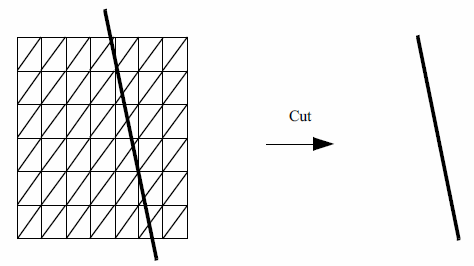
\includegraphics[width=0.98\textwidth]{Figure9-6}\\
    \caption{Cutting polygons produces lines (cutPlane.tcl).}\label{fig:Figure9-6}
\end{figure}

\begin{figure}[!htb]
    \centering
    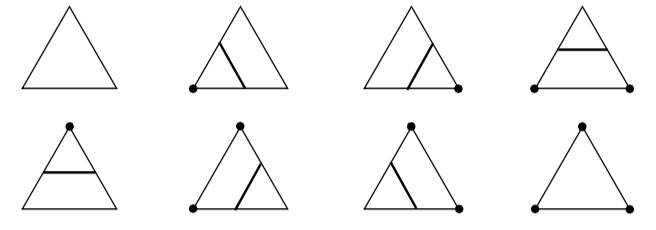
\includegraphics[width=0.98\textwidth]{Figure9-7}\\
    \caption{The eight cases for cutting (contouring) a triangle. Black dots show triangle vertices that are ``inside'' the scalar cutting region. Solid lines show the output of the cutting operation.}\label{fig:Figure9-7}
\end{figure}

We can do clipping with arbitrary implicit functions using a variation of the ``marching'' primitives discussed in ``Contouring''on page \ref{subsec:contouring}. We illustrate the technique for triangles.

Recall that marching triangles transforms triangles into lines that approximate a scalar value called the isovalue. This is accomplished using the inside/outside relationship that each vertex has with respect to some scalar value. For our purposes here, we use a scalar value that represents the signed distance of the triangle vertex to a plane. This infinite plane, described by an implicit function of the form $F(x, y, z) = n_{xx} + n_{yy} + n_{zz} - d = 0$, partitions space into two infinite half spaces. All points with negative scalar values lie on one side of the plane and all with positive values lie on the other side. Figure \ref{fig:Figure9-6} shows a finite plane represented by a grid of triangles. The thick line shows the infinite plane defined by $F(x,y,z) = x + y + z - c = 0$. The cut algorithm described in ``Cutting'' on page \pageref{subsec:cutting} creates a set of lines using the contour operations specific to each cell primitive. In this example, the triangle's contour operator extracts lines that lie on the intersection of the infinite plane and the triangles that comprise the finite plane. The contour operation for a triangle uses the eight cases shown in Figure \ref{fig:Figure9-7} to contour or ``cut'' each triangle appropriately.

\begin{figure}[!htb]
    \centering
    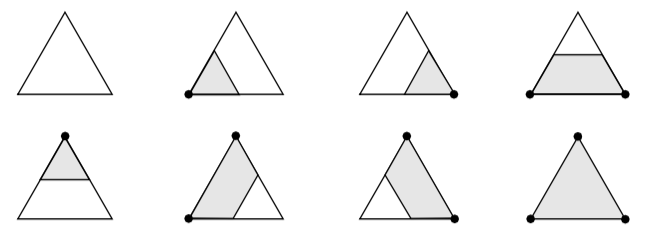
\includegraphics[width=0.98\textwidth]{Figure9-8}\\
    \caption{The eight cases for clipping a triangle. Black dots show triangle vertices that are "inside" the scalar clipping region. Shaded regions show the output of the clip operation.}\label{fig:Figure9-8}
\end{figure}

\begin{figure}[!htb]
    \centering
    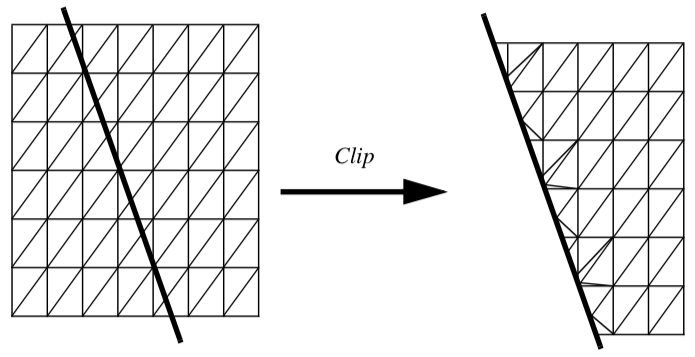
\includegraphics[width=0.98\textwidth]{Figure9-9}\\
    \caption{A plane of triangles clipped with a plane function (clipPlane.tcl).}\label{fig:Figure9-9}
\end{figure}

Clipping transforms polygons into polygons. We do clipping with a modified case table for the triangle that outputs polygons shown in Figure \ref{fig:Figure9-8}. In VTK, each polygonal data cell has a different case table to define the clip operation. Applying the clip algorithm to the polygonal data in Figure \ref{fig:Figure9-9} using the same scalar field generated with a plane equation produces a new set of triangles.

Formulating clipping using scalar fields permits more sophisticated operations. Clipping can use scalar data that is computed or scalar data that is part of a polygonal dataset's point attributes.

\begin{figure}[!htb]
    \centering
    \begin{subfigure}{0.41\linewidth}
        \centering
        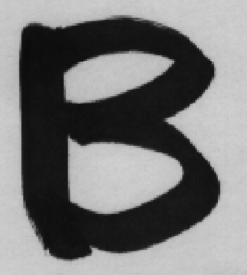
\includegraphics[width=.96\linewidth]{Figure9-10a}
        \caption*{}\label{fig:Figure9-10a}
    \end{subfigure}
    \hfill
    \begin{subfigure}{0.16\linewidth}
        \centering
        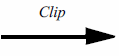
\includegraphics[width=.96\linewidth]{Figure9-10b}
        \caption*{}\label{fig:Figure9-10b}
    \end{subfigure}%
    \hfill
    \begin{subfigure}{0.41\linewidth}
        \centering
        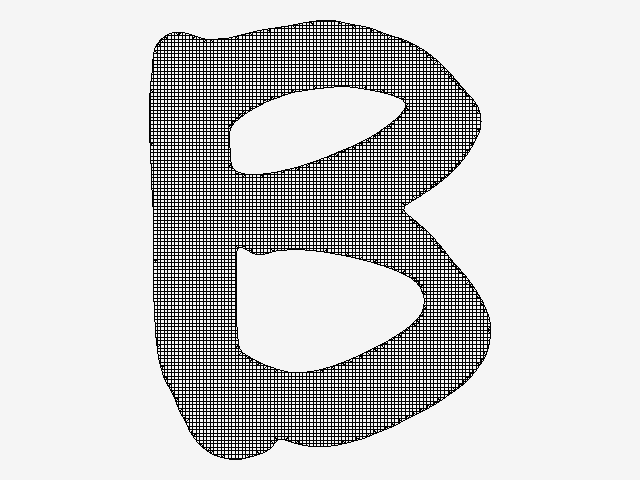
\includegraphics[width=.96\linewidth]{Figure9-10c}
        \caption*{(\href{https://lorensen.github.io/VTKExamples/site/Cxx/VisualizationAlgorithms/CreateBFont/}{CreateBFont.cxx} or \href{https://lorensen.github.io/VTKExamples/site/Python/VisualizationAlgorithms/CreateBFont/}{CreateBFont.py})}\label{fig:Figure9-10c}
    \end{subfigure}%
    \caption{Carpet plot. (a) Visualization of an exponential cosine function. Function values are indicated by surface displacement. Colors indicate derivative values. Carpet plot of combustor flow energy in a structured grid. Colors and plane displacement represent energy values.}
    \label{fig:Figure9-10}
\end{figure}

Figure \ref{fig:Figure9-10} shows a scanned image that is first converted to a quadrilateral mesh with vertex scalar values set to the scanned image intensity. Clipping this quadrilateral mesh with a value equal to 1/2 the maximum intensity of the scanned image produces a polygonal model show in Figure \ref{fig:Figure9-10}.

\section{Vector Algorithms}

\subsection{Vector Field Topology}

\begin{figure}[htb]
	\begin{subfigure}[h]{0.32\linewidth}
		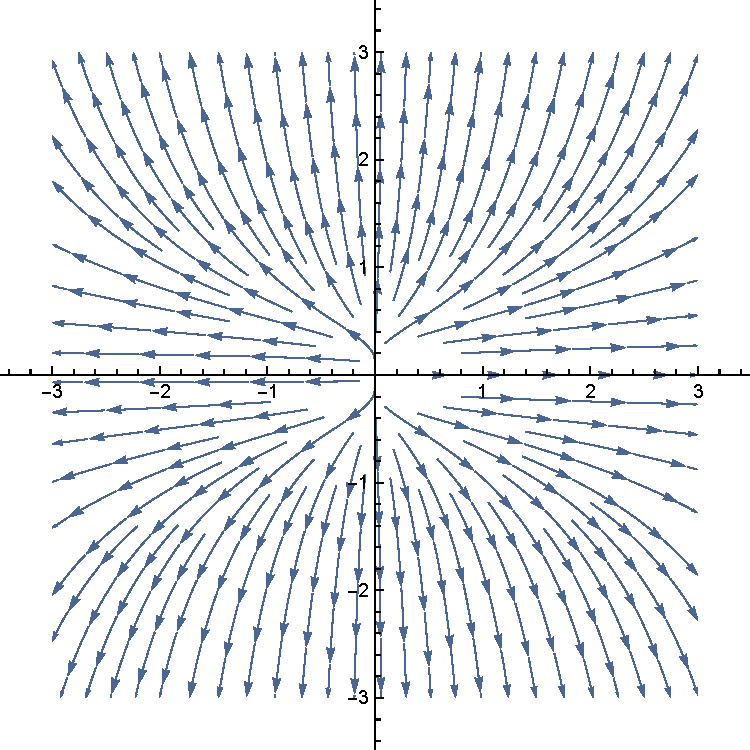
\includegraphics[width=0.86\linewidth]{Figure9-13a}
		\captionsetup{justification=centering}
		\caption*{Repelling Node\\$R_1, R_2 > 0$\\$I_1, I_2 = 0$}
		\label{fig:Figure9-13a}
	\end{subfigure}
	\hfill
	\begin{subfigure}[h]{0.32\linewidth}
		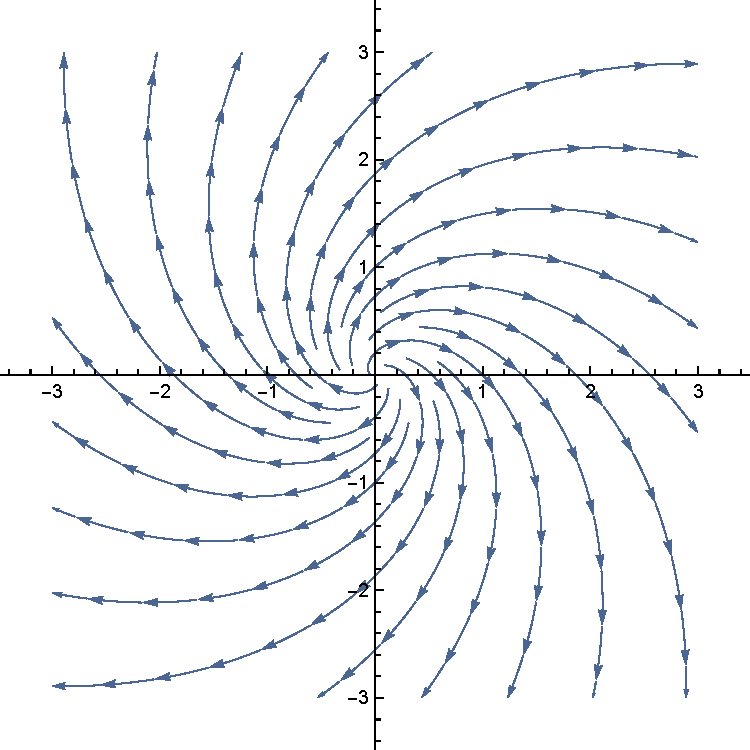
\includegraphics[width=0.86\linewidth]{Figure9-13b}
		\captionsetup{justification=centering}
		\caption*{Repelling Focus\\$R_1, R_2 > 0$\\$I_1, I_2 \neq 0$}
		\label{fig:Figure9-13b}
	\end{subfigure}
	\hfill
	\begin{subfigure}[h]{0.32\linewidth}
		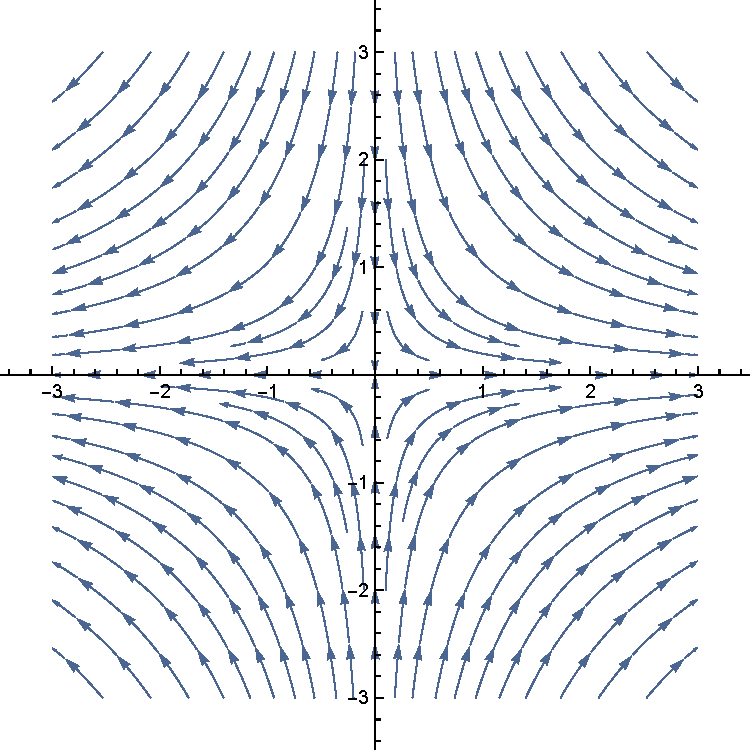
\includegraphics[width=0.86\linewidth]{Figure9-13c}
		\captionsetup{justification=centering}
		\caption*{Saddle Point\\$R_1 \times R_2 < 0$\\$I_1, I_2 = 0$}
		\label{fig:Figure9-13c}
	\end{subfigure}
	\hfill
		\begin{subfigure}[h]{0.32\linewidth}
		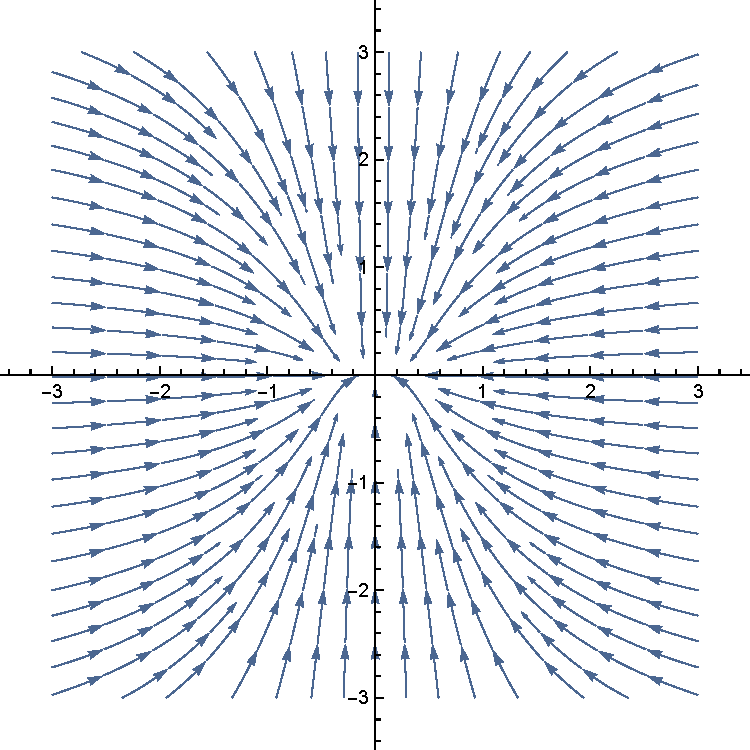
\includegraphics[width=0.86\linewidth]{Figure9-13d}
		\captionsetup{justification=centering}
		\caption*{Attracting Node\\$R_1, R_2 < 0$\\$I_1, I_2 = 0$}
		\label{fig:Figure9-13d}
	\end{subfigure}
	\hfill
	\begin{subfigure}[h]{0.32\linewidth}
		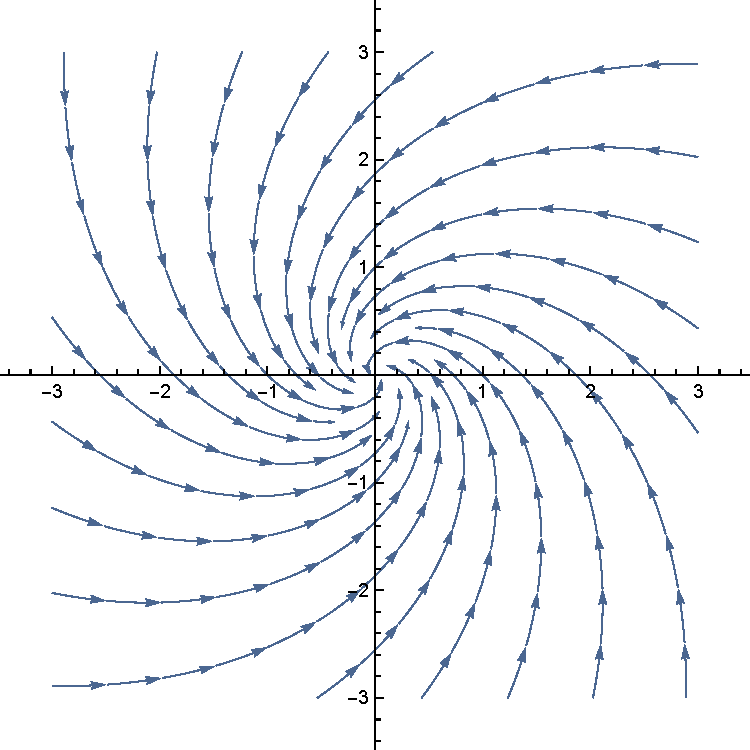
\includegraphics[width=0.86\linewidth]{Figure9-13e}
		\captionsetup{justification=centering}
		\caption*{Attracting Focus\\$R_1, R_2 < 0$\\$I_1, I_2 \neq 0$}
		\label{fig:Figure9-13e}
	\end{subfigure}
	\hfill
	\begin{subfigure}[h]{0.32\linewidth}
		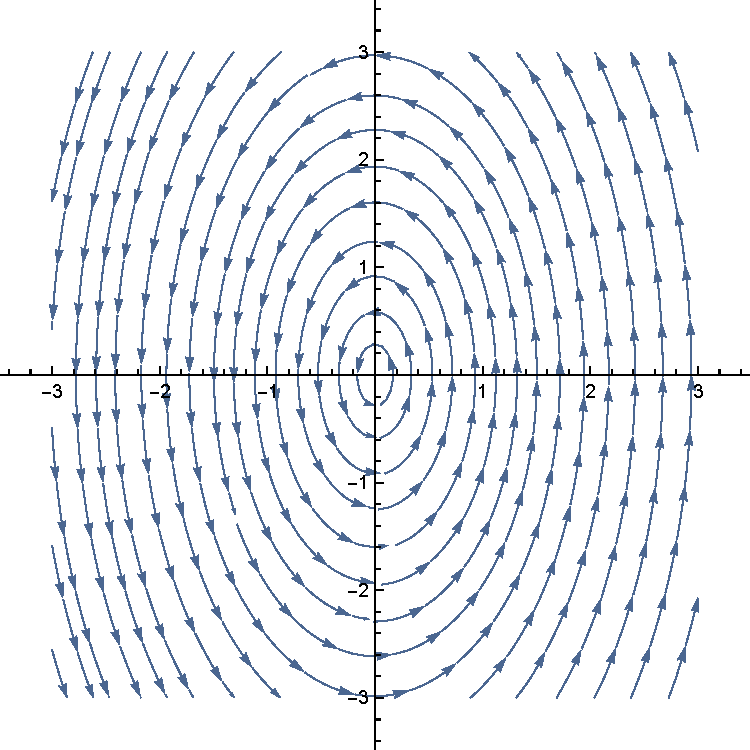
\includegraphics[width=0.86\linewidth]{Figure9-13f}
		\captionsetup{justification=centering}
		\caption*{Center\\$R_1, R_2 = 0$\\$I_1, I_2 \neq 0$}
		\label{fig:Figure9-13f}
	\end{subfigure}
	\caption{Critical points in two dimensions. The real part of the eigenvalues ($R_1$, $R_2$) of the matrix of first derivatives control the attraction or repulsion of the vector field. The imaginary part of the eigenvalues ($I_1$, $I_2$) controls the rotation.}\label{fig:Figure9-13}
\end{figure}


\begin{equation}\label{eq:9.12}
H_d = \overrightarrow{v\ } \cdot \overrightarrow{w\ } = \vert \overrightarrow{v\ } \vert \vert \overrightarrow{w\ } \vert \cos(\phi)
\end{equation}
\myequations{Scalar function of the vector dot product. }

\section{Tensor Algorithms}

\section{Modelling Algorithms}

\subsection{Decimation}

\begin{description}
	\item[Triangulation.] \label{subsec:decimation.triangulation} After deleting a point, the resulting hole must be retriangulated.
\end{description}

\subsection{Mesh Smoothing}
\label{subsec:mesh_smoothing}

\subsection{Visualizing Unstructured Points}
\label{subsec:visualizing_unstructured_points}

\subsection{Texture Algorithms}
\label{subsec:texture_algorithms}

\section{Putting It All Together}

\subsection{Connectivity}
\label{subsec:connectivity}

\section{Chapter Summary}

Dividing cubes is a scalar contouring operation that generates points rather than surface primitives such as lines or polygons. Dense point clouds appear solid because of the limited resolution of computer images.

Vector fields have a complex structure. This structure can be visualized using streamribbons, streamsurfaces, and streampolygons. The topology of a vector field can be characterized by connecting critical points with streamlines.

Tensor fields consist of three orthogonal vector fields. The vector fields are the major, medium, and minor eigenvectors of the tensor field. Hyperstreamlines can be used to visualize tensor fields.

Dataset topology operations generate triangle strips, extract connected surfaces, and compute surface normals. Decimation is a polygon reduction algorithm that reduces the number of triangles in a triangle mesh. Implicit modelling techniques can be used to construct swept surfaces and volumes. Unstructured points are easy to represent but difficult to visualize. Splatting, interpolation, and triangulation techniques are available to construct structure for unstructured points. Multivariate visualization is required for data of dimension four and higher. Data must be mapped to three dimensions before standard visualization techniques can be used. Parallel coordinates techniques are also available to visualize multivariate data.

Modelling algorithms extract geometric structure from data, reduce the complexity of the data or create geometry. Spatial extraction selects dataset structure and associated data attributes lying within a specified region in space. Subsampling reduces data by selecting every nth data point. A related technique, data masking, selects every nth cell. Subsets of a dataset can also be selected using thresholding, which selects cells or points that lie within a range of scalar values. Probing resamples data at a set of points. The probe produces a dataset that has the topology of the probe with data values from the probed dataset. Generating triangle strips can reduce storage requirements and improve rendering speeds on some systems. If a dataset has multiple disjoint structures, a connectivity algorithm can uniquely identify the separate structures. For polygonal data that does not have vertex normals defined, normal generation algorithms can compute these values that are suitable for interpolation by Gouraud or Phong shading. Decimation, another data reduction technique, removes triangles in ``flat'' regions and fills the resulting gaps with new triangles. Unstructured points present a challenge because the data does not have topology. Splatting represents each point in the data with a uniform sampling and accumulates these splats using implicit modelling techniques. Triangulation techniques build topology directly from the unstructured points.

Multidimensional visualization techniques focus on data that has many scalar data values for each point. Parallel coordinates is an interesting approach that plots the scalar values for a data point along a parallel axis. The observer looks for trends and relationships between the lines that represent each point's data.

Texture algorithms use texture coordinates and texture maps to select or highlight portions of a dataset. Texture thresholding assigns texture coordinates based on a scalar value. The scalar value and texture map determine how a cell or portion of a cell is rendered. Boolean textures extend this concept to 2D and 3D. Careful design of a boolean texture map permits the ``clipping'' of geometry with combinations of implicit surfaces. Texture can also be used to animate vector fields.

\section{ Bibliographic Notes}

Dividing cubes is an interesting algorithm because of the possibilities it suggests \cite{Cline88}. Point primitives are extremely simple to render and manipulate. This simplicity can be used to advantage to build accelerated graphics boards, perform 3D editing, or build parallel visualization algorithms.

Many plotting and visualization systems use carpet plots extensively. Carpet plots are relatively easy to represent and render. Often 2D plotting techniques are used (i.e., lighting and perspective effects ignored). Check \cite{Wang90} for additional information on rendering carpet plots.

In recent years a number of powerful vector visualization techniques have emerged. These techniques include streamsurfaces \cite{Hultquist92}, streampolygons \cite{Schroeder91}, vector field topology \cite{Helman91} \cite{Globus91}, streamballs \cite{Brill94}, and vorticity visualization \cite{Banks94}. The streamballs technique is a recent technique that combines techniques from implicit modeling. You may also wish to see references \cite{Crawfis92} \cite{vanWijk93} and \cite{Max94}. These describe volume rendering and other advanced techniques for vector visualization, topics not well covered in this text.

Some abstract yet beautiful visualization images are due to Delmarcelle and Hesselink \cite{Delmarcelle93}. Their rendering of hyperstreamlines reflect the underlying beauty and complexity of tensor fields.

Polygon reduction is a relatively new field of study. SIGGRAPH '92 marked a flurry of interest with the publication of two papers on this topic \cite{Schroeder92a} \cite{Turk92}. Since then a number of valuable techniques have been published. One of the best techniques, in terms of quality of results, is given by \cite{Hoppe93}, although it is limited in time and space because it is based on formal optimization techniques. Other interesting methods include \cite{Hinker93} and \cite{Rossignac93}. A promising area of research is multiresolution analysis, where wavelet decomposition is used to build multiple levels of detail in a model \cite{Eck95}. The most recent work in this field stresses progressive transmission of 3D triangle meshes \cite{Hoppe96}, improved error measures \cite{Garland97}, and algorithms that modify mesh topology \cite{Popovic97} \cite{Schroeder97}. Most recently an extensive book on the technology is available including specialized methods for terrain simplification \cite{Luebke02}.

Triangle strip generation is an effective technique for achieving dramatic improvements in rendering speed and reductions in data handling. The reference by \cite{Evans96} describes other triangle strip generation algorithms as well as presenting some of the most effective techniques to date.

The use of texture for visualization is relatively unexploited. This has been due in part to lack of texture support in most graphics software and hardware. This is now changing, as more vendors support texture and software systems (such as OpenGL) that provide an API for texture. Important references here include the boolean textures \cite{Lorensen93} and surface convolution techniques \cite{Cabral93} \cite{Stalling95}.

Unstructured or unorganized point visualization is likely to play a prominent role in visualization as the field matures and more complex data is encountered. Nielson et al. have presented important work in this field \cite{Nielson91a}.

Multidimensional visualization is another important focus of visualization research \cite{Bergeron89} \cite{Mihalisin90}. Much real-world data is both unstructured and multidimensional. This includes financial databases, marketing statistics, and multidimensional optimization. Addressing this type of data is important to achieve future advances in understanding and application. Feiner \cite{Feiner90} has presented a simple projection method combined with virtual reality techniques. \cite{Inselberg87} has introduced parallel coordinates. These techniques have been shown to be powerful for many types of visual analysis.

\printbibliography

\section{Exercises}

\begin{enumerate}

\item Describe an approach to adapt dividing cubes to other 3D cell types. Can your method be adapted to 1D and 2D cells?

\item Discuss the advantages and disadvantages of representing surfaces with points versus polygons.

\item Streamribbons can be constructed by either i) connecting two adjacent streamlines with a surface, or ii) placing a ribbon on the streamline and orienting the surface according to streamwise vorticity vector. Discuss the differences in the resulting visualization.

\item Write the following programs to visualize velocity flow in the combustor.

    \begin{enumerate}

    \item Use vtkProbeFilter and vtkHedgeHog.

    \item Use vtkProbeFilter and vtkStreamLine.

    \item Use vtkProbeFilter and vtkWarpVector.

    \item Use vtkProbeFilter and vtkVectorNorm.

    \item Use vtkProbeFilter and vtkVectorDot.

    \end{enumerate}

\item Describe a method to extract geometry using an arbitrary dataset. (That is, extract geometry that lies within the culling dataset.) (Hint: how would you evaluate in/out of points?)

\item The filter vtkPolyDataNormals is often used in combination with the filters vtkSmoothPolyData and vtkContourFilter to generate smooth isosurfaces.

    \begin{enumerate}

    \item Write a class to combine these three filters into one filter. Can you eliminate intermediate storage?

    \item How much error does vtkSmoothPolyData introduce into the isosurface? Can you think of a way to limit the error?

    \item What is the difference between the surface normals created by vtkMarchingCubes and vtkPolyDataNormals?

    \end{enumerate}

\item Assume that we have a database consisting of interest rate R, monthly payment P, monthly income I, and days payment is late L.

    \begin{enumerate}

    \item If R, P, I are all sampled regularly, how would you visualize this data?

    \item If all data is irregularly sampled, list three methods to visualize it.

    \end{enumerate}

\item Why do you think triangle strips are often faster to render than general polygons?

\item The normal generation technique described in this chapter creates consistently oriented surface normals.

    \begin{enumerate}

    \item Do the normals point inside or outside of a closed surface?

    \item Describe a technique to orient normals so that they point out of a closed surface.

    \item Can surface normals be used to eliminate visible triangles prior to rendering? (Hint: what is the relationship between camera view and surface normal?)

    \end{enumerate}

\item Describe a technique to partially threshold a cell (i.e., to cut a cell as necessary to satisfy threshold criterion). Can an approach similar to marching cubes be used?

\item The class vtkRendererSource allows us to use the rendered image as a texture map (or image data dataset). Write a program to construct iterated textures, that is textures that consist of repeated images. Can the same image be generated using texture coordinates?

\item Describe how you would modify the decimation algorithm to treat general polygons.

\item Several examples in the text (e.g., deciFran.tcl and deciHawa.tcl) use the class vtkDecimate. Modify these examples to use the topology modifying progressive decimation algorithm (implemented in vtkDecimatePro). How much greater reduction can you achieve?


\end{enumerate}